\documentclass[10pt]{article}
\usepackage{../../local}
\urlstyle{same}

\newcommand{\classcode}{EE 120}
\newcommand{\classname}{Signals and Systems}
\renewcommand{\maketitle}{%
\hrule height4pt
\large{Eric Du \hfill \classcode}
\newline
\large{HW 03} \Large{\hfill \classname \hfill} \large{\today}
\hrule height4pt \vskip .7em
\small{Header styling inspired by CS 70: \url{https://www.eecs70.org/}}
\normalsize
}
\linespread{1.1}
\begin{document}
	\maketitle
	\section*{Collaborators}
	I worked with the following people to complete this assignment:
	\begin{itemize}
		\item Teja Nivarthi: 
		\item Nikhil Maserang:
	\end{itemize}
	\pagebreak
	\section*{Problem 1}
	Here is a list of statements about systems. Determine if each of them is true or false with your justification. 
	\begin{enumerate}[label=\alph*)]
		\item If an LTI system is causal, it's stable. 

			\begin{solution}
				False. A system being causal -- the fact that it only depends on past inputs, has nothing to do 
				with whether it is bounded or not.
			\end{solution}
		\item If a discrete time LTI system has an impulse response \( h[n] \) of finite duration, the system 
			is stable. 

			\begin{solution}
				Based on Ed, we are allowed to assume that \( h[n] \) also has finite amplitude. Then, we know 
				that the signal response for an LTI system is characterized by the convolution of the impulse 
				response with \( x[n] \) :
				\[
					y[n] = x[n] * h[n] = \sum_{k = -\infty}^{\infty} x[k] h[n-k] 
				\] 
				If \( x[n] \) is bounded and \( h[n]  \) is bounded, then we know that the system is stable. 
				Alternatively, one could argue this by using the fact that \( h[n] \) is absolutely 
				integrable, so it is stable. 
			\end{solution}
		\item If \( h(t) \) is the impulse response of an LTI system and \( h(t) \) is periodic and non-zero, the 
			system is unstable. 

			\begin{solution}
				True. If \( h(t) \) is nonzero and nonperiodic, then it is not absolutely integrable. Hence, it cannot 
				be stable.
			\end{solution}
		\item If \( |h[n]| \le K \) for each \( n \), where \( K \) is a given number, then the LTI system with 
			\( h[n] \) as its impulse response is stable. 

			\begin{solution}
				False. If \( h[n] \) does not have finite support, then an LTI system with \( h[n] \) as its impulse
				response is still not absolutely integrable, so the system is not stable.
			\end{solution}
		\item A discrete-time LTI system is causal if and only if its step response \( s[n] \) is 
			zero for \( n < 0 \). 

			\begin{solution}
				True. An LTI system is causal if and only if its impulse response is a causal function (i.e. 
				it's value is 0 for all \( t < 0 \)), which is true in this case.  
			\end{solution}
	\end{enumerate}
	\pagebreak
	\section*{Problem 2}
	Here are some impulse responses \( h[n] \) and \( h(t) \) of several discrete-time and continuous-time LTI systems, 
	where \( u[n] \) and \( u(t) \) are the discrete-time and continuous-time unit step functions, respectively.
	Determine wheter each system is 1) stable or not, 2) causal or not. Show your justification.
	\begin{enumerate}[label=\alph*)]
		\item \( h[n] = \alpha^{n}u[n] \) for \( |\alpha| < 1 \)

			\begin{solution}
				The function \( h[n] \) is absolutely summable (it's a geometric series over \( \alpha \), and since 
				\( |\alpha| < 1 \) then the series converges), so it is stable. It is also causal, since the 
				impulse response is causal. 
			\end{solution}
		\item \( h[n] = \beta^{n} u[3 - n] \) for \( |\beta| > 1 \)

			\begin{solution}
				This system is also absolutely summable -- it's the same geometric series as in (a) except it's 
				support is over the interval \( (-\infty, 3] \). Therefore, it is stable. It is not causal, however
				since \( h[n] \neq 0  \) for  \( n < 0 \). 
			\end{solution}
		\item \( h(t) = e^{-4t|t|} \)

			\begin{solution}
				This function is in fact absolutely integrable: for \( t > 0 \), the function \( h(t) = e^{-4t^2} \), 
				which converges over the interval \( [0, \infty) \). For \( t < 0 \), then we have 
				\( |t| = -t \), so therefore \( h(t) = e^{4t^2} \), which is also absolutely integrable over 
				the interval \( (-\infty, 0] \). Therefore, since \( h(t)  \) is absolutely integrable over 
				the whole space \( (-\infty, \infty) \), then we know that \( h(t) \) is absolutely integrable, 
				hence it is BIBO stable. 

				The system is not causal however, since \( h(t)  \) is nonzero for \( t < 0 \).
			\end{solution}
		\item \( h(t) = te^{-t}u(t) \)

			\begin{solution}
				For \( t > 0 \), this function is \( h(t) = te^{-t} \), 
				and computing the integral on \( [0, \infty) \):
				\[
					\int_{0}^{\infty} |h(t)| dt = \int_{0}^{\infty} te^{-t}dt =1  
				\] 
				(I used mathematica because I'm lazy.) \( h(t) = 0 \) for \( t < 0 \), so \( h(t) \) is 
				absolutely summable, hence it is BIBO stable.

				The system is also causal because for \( t < 0 \) we have \( h(t) < 0 \). 
			\end{solution}
	\end{enumerate}
	\pagebreak
	\section*{Problem 3}
	Consider the cascade of two LTI systems:
	\begin{center}
		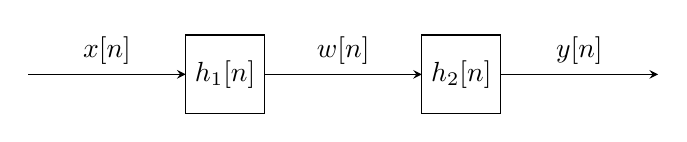
\begin{tikzpicture}
			\draw[-stealth] (-3, 0) -- node[midway, above] {\( x[n] \) } (-1, 0); 
			\draw (-1, -0.5) rectangle node{\( h_1[n] \) } (0, 0.5);
			\draw[-stealth] (0, 0) -- node[midway, above] {\( w[n] \) } (2, 0);
			\draw(2, -0.5) rectangle node {\( h_2[n] \) } (3, 0.5);
			\draw[-stealth] (3, 0) -- node[midway, above] {\( y[n] \) }  (5, 0);
		\end{tikzpicture}
	\end{center}
		where we have 
		\[
			h_1[n] = \sin[8n]
		\] 
		and 
		\[
			h_2[n] = a^{n}u[n] \ \ |a| < 1
		\] 
		and the input is
		\[
			x[n] = \delta[n] - a \delta[n - 1] 
		\] 
		Determine the output \( y[n] \) using convolution properties. \textit{Hint:} Use the commutative property of 
		convolution.

		\begin{solution}
			We know that for two LTI systems in series, then the signal output  \( y[n] \) is defined as 
			\[
				y[n] = (x[n] * h_1[n]) * h_2[n] = x[n] * (h_2[n] * h_1[n]) = (x[n] * h_2[n]) * h_1[n]
			\] 
			where we've used both associativity and commutativity. Now we just carry out the algebra: 
			\begin{align*}
				y[n] &= \left( \sum_{k = -\infty}^{\infty}x[n - k] h_2[k] \right) *h_1[n] \\
					 &= \left( \sum_{k = -\infty}^{\infty}(\delta[n - k] - a\delta[n - k - 1]) a^{k}u[k] \right) *h_1[n] \\
					 &= \underbrace{\left[ a^{n}u[n] - a^{n}u[n -1] \right]}_{a^{n}\delta[n]} * h_1[n]  \\
					 &= \sum_{k = -\infty}^{\infty}a^{n - k}\delta[n - k] \sin[8n] \\
					 &= \sin[8n] 
			\end{align*}
			so we have \( y[n] = h_1[n] = \sin[8n] \), what a wonderful coincidence. 
		\end{solution}
	\pagebreak
	\section*{Problem 4}
	This problem will explore the connection between LCCDEs and the frequency response. The LCCDE for system \( F \) 
	is
	\[
		3y[n] - 4y[n - 1] - 5y[n -2]  = 6x[n] + 7x[n-1] \ \forall n \in \mathbb Z
	\] 
	\begin{enumerate}[label=\alph*)]
		\item Using the eigenfunction property, find the frequency response \( F( \omega) \).

			\begin{solution}
				The Eigenfunction property says that given a signal  \( x[n] = Ae^{i \omega n} \), then the 
				output signal \( y[n] = F(\omega)x[n]\). Using this property, we can write:
				\begin{align*}
					3F(\omega) Ae^{i \omega n } - 4F(\omega) Ae^{i \omega (n - 1)} - 5F(\omega) Ae^{ i \omega (n - 2)}
					&= 6Ae^{ i \omega n} + 7Ae^{i \omega (n -1)} \\
					F(\omega)\left( 4e^{i \omega n} - 5e^{i \omega (n - 1)} - 5e^{i \omega (n - 2)} \right) 
					&= e^{i \omega(n -1)}(6e^{i \omega} + 7)
				\end{align*}
				Isolating for \( F(\omega)  \) gives:
				\[
				F(\omega) = \frac{e^{i \omega(n - 1)(6e^{i \omega} + 7)}}{e^{i \omega(n - 2) (3e^{2 i \omega} - 
				4e^{i \omega} - 5}} = \frac{e^{i \omega}(6e^{i \omega} + 7)}{3e^{2 i \omega} - 4e^{ i \omega} - 5}
				\] 
			\end{solution}
		\item Now given a general LCCDE in this form:
			\[
				a_0y[n] + a_1y[n -1] + \cdots + a_k y[n -k] = b_0x[n] + b_1x[n -1] + \cdots + b_l x[n -l]
			\] 
			Find the frequency response \( F(\omega) \). 

			\begin{solution}
				Following the pattern derived in the previous part, we then know that: 
				\[
				F(\omega) = \frac{\sum_{m = 0}^{l} b_me^{-i \omega m}}{\sum_{m = 0}^{k}a_m e^{-i \omega m}}
				\] 
			\end{solution}
		\item Based on your results from above, find the LCCDE given the frequency response for a new LTI system 
			H. 
			\[
			H(\omega) = \frac{3 + 8e^{3i \omega} - e^{5i\omega}}{1 + e^{i \omega}}
			\] 

			\begin{solution}
				Based on this, we can conclude that \( b_i = \{3, 0, 0, 8, 0, -1\}  \), and 
				\( a_i = \{1, 1\}  \). Therefore: 
				\[
					y[n] + y[n - 1] = 3x[n] + 8x[n - 3] - x[n - 5]
				\] 
			\end{solution}
	\end{enumerate}
	\pagebreak
	\section*{Problem 5}
	The following input signal is applied to a real, continuous-time LTI system: 
	\begin{align*}
		x&: \R \to \R\\
		\forall t &\in \R, \ \ \ x(t) = \begin{cases}
			1 & \text{if \( |t| \le \frac{1}{2} \)}\\
			0 & \text{elsewhere}
		\end{cases}
	\end{align*}
	For each LTI system described below, determine the output signal \( y \) in response to the input 
	signal \( x \); do this by providing a well-labeled plot of \( y \) as a function of \( t \) or finding 
	an expression for \( y \) in terms of \( x \). 
	\begin{enumerate}[label=\alph*)]
		\item The impulse response \( h \) of the LTI system is 
			\begin{align*}
				h &: \R \to \R\\
				\forall t &\in \R \ \ \  h(t) = \begin{cases}
					1 & \text{if \( 1 \le  t \le  2 \)}\\
					0 & \text{elsewhere}
				\end{cases}
			\end{align*}

			\begin{solution}
				We use the formula for the convolution:
				\[
				y(t) = x(t) * h(t) = \int_{-\infty}^{\infty} x(\tau) h(t - \tau) \diff \tau 
				\] 
				We know that \( x(t) \) is only nonzero on the interval \( [-\frac{1}{2}, \frac{1}{2}] \), so 
				we restrict \( \tau \) to this interval. Further, since \( x(t) \) is constant, we can use that 
				to siplify the expression too:
				\[
					y(t) = \int_{-\frac{1}{2}}^{\frac{1}{2}} h(t - \tau) \diff \tau 
				\] 
				Consider a particular \( t \). Then, the integral sweeps over a region of \( t - \frac{1}{2} \) to 
				\( t + \frac{1}{2} \). Since  \( h(t) \) is nonzero on \( [1, 2] \), this means that for any 
				\( t < \frac{1}{2} \) or \( t > \frac{5}{2} \), we have \( y(t) = 0 \). Then, for 
				\( \frac{1}{2} < t < \frac{3}{2} \), then our integral goes from 1 to \( t + \frac{1}{2} \): 
				\[
				y(t) = \int_{1}^{t + \frac{1}{2}} h(\tau)\diff \tau = t-\frac{1}{2}
				\] 
				Then, for \( \frac{3}{2} < t < \frac{5}{2} \), the integral goes from \( t - \frac{1}{2} \) to 
				\( 2 \) :
				\[
				y(t) = \int_{t - \frac{1}{2}}^{2} h(\tau) \diff \tau =  -t + \frac{5}{2}
				\] 
				So in essence, \( y(t) \) is a triangle function. Written out explicitly, we have: 
				\[
				y(t) = \begin{cases}
					0 & \text{\( t < \frac{1}{2} \) or \( t > \frac{5}{2} \)}\\
					t - \frac{1}{2} & \frac{1}{2} < t < \frac{3}{2}\\
					\frac{5}{2} - t & \frac{3}{2} < t < \frac{5}{2}
				\end{cases}
				\] 
				Plotting: 
				\begin{center}
					\includegraphics[scale=0.8]{q5a.png}
				\end{center}
			\end{solution}
		\item the impulse response \( h \) of the LTI system is
			\begin{align*}
				h &: \R \to \R\\
				\forall t &\in \R, \ \ \ h(t) = \begin{cases}
					1 & \text{if \( 1 \le t \le 3 \)}\\
					0 & \text{elsewhere}
				\end{cases}
			\end{align*}

			\begin{solution}
				This is very similar to the previous problem esxcept our limits are different. 
				For \( t < \frac{1}{2} \) and \( t > \frac{7}{2} \), we have \( y(t) = 0 \). For 
				\( \frac{1}{2} < t < \frac{3}{2} \), the integral is the same, over the interval \( 1\) to 
				\( t + \frac{1}{2} \)
				\[
				y(t) = \int_{1}^{t + \frac{1}{2}} h(\tau) \diff \tau = t - \frac{1}{2} 
				\] 
				For \( \frac{3}{2} < t < \frac{5}{2} \), \( h(t) \) is constant on this interval, so the 
				value over this interval is just the area under a rectangle of width 1 and height 1:
				\[
				y(t) = \int_{t-\frac{1}{2}}^{t+\frac{1}{2}} h(\tau)\diff \tau = 1
				\] 
				For \( \frac{5}{2} < t < \frac{7}{2} \), our integral goes from \( t - \frac{1}{2} \) to \( 3 \), 
				so therefore: 
				\[
				y(t) = \int_{t-\frac{1}{2}}^{3} h(\tau)\diff \tau = \frac{7}{2} - t 
				\] 
				Therefore, we have: 
				\[
				y(t) = \begin{cases}
					0 & \text{\( t<\frac{1}{2} \) or \( t > \frac{7}{2} \)}\\
					t - \frac{1}{2} & \frac{1}{2} < t < \frac{3}{2}\\
					1 & \frac{3}{2} < t < \frac{5}{2}\\
					\frac{7}{2} - t & \frac{5}{2} < t < \frac{7}{2}
				\end{cases}
				\] 
				Plotting: 
				\begin{center}
					\includegraphics[scale=0.8]{q5b.png}
				\end{center}
			\end{solution}
		\item The impulse response \( h \) of the LTI system is 
			\begin{align*}
				h&: \R \to \R\\
				\forall t &\in \R, \ \ \ h(t) = \delta(t) - \delta\left( t - \frac{1}{2} \right) 
			\end{align*}
			where \( \delta \) is the Dirac delta function.

			\begin{solution}
				We know that convolutions are distributive: 
				\[
				y(t) = x(t) * h(t) = x(t) * \left[ \delta(t) - \delta\left( t - \frac{1}{2} \right)  \right] 
				= x(t) * \delta(t) - x(t) * \delta\left( t - \frac{1}{2} \right) 
				\] 
				Then, we use the identity that \( x(t) * \delta(t - T) = x(t - T) \). Therefore, we have: 
				\[
				y(t) = x(t) - x\left(t - \frac{1}{2}\right)
				\] 
			\end{solution}
		\item The impulse response \( h \) of the LTI system is 
			\begin{align*}
				h&: \R \to \R\\
				\forall t &\in \R \ \ \ h(t) = \sum_{k = -\infty}^{\infty}\delta (t - kT)
			\end{align*}
			where \( 1 < T \). 

			\begin{solution}
				This is a generalization of the previous part,so we have: 
				\[
				y(t) = x(t) * \sum_{k = -\infty}^{\infty} \delta(t - kT) = \sum_{k = -\infty}^{\infty}x(t - kT)
				\] 
				Since \( T > 1 \), this function basically is a series of square pulses separated \( T \) apart 
				from one another. Since we're not given a value of \( T \), it's impossible to plot it. 
			\end{solution}
	\end{enumerate}
	\pagebreak
	\section*{Problem 6}
	Consider the signal 
	\[
		x[n] = \alpha ^{n}u[n]
	\] 
	\begin{enumerate}[label=\alph*)]
		\item Sketch the signal \( g[n] = x[n] - \alpha x[n -1] \). Write \( g[n] \) as a convolution related 
			to \( x[n] \). 

			\begin{solution}
				Firstly, to plot \( g[n] \), we simplify the expression for \( g \) :
				\begin{align*}
					g[n] &= x[n] - \alpha x[n -1] \\
						 &= \alpha ^{n} u[n] - \alpha ^{n}u[n-1]\\
						 &= \alpha ^{n}(u[n] - u[n -1] )\\
						 &= \alpha ^{n} \delta[n] 
				\end{align*}
				So this is basically a delta function with height \( \alpha ^{n} \) at \( n = 0 \), and zero 
				everywhere else. Plotting this: 
				\begin{center}
					\begin{tikzpicture}
						\draw (-3, 0) -- (3, 0) node[right] {\( n \) };
						\draw (0, -3) -- (0, 3) node[above] {\( g[n] \) };
						\foreach \x in {-3, -2, -1, 1, 2, 3}
						\filldraw[red] (\x, 0) circle (0.5mm); 
						\draw[red, thick] (0, 0) -- (0, 2.5);
						\filldraw[red] (0, 2.5) circle (0.5mm) node[right] {\( \alpha^n \) };
					\end{tikzpicture}
				\end{center}
				Now, we write \( g[n] \) as a convolution related to \( x[n] \). To do this, we go back to the original 
				form of \( g[n] = x[n] - \alpha x[n - 1] \). Becuase we want to write \( g[n] = x[n] * h[n] \) for 
				some \( h[n] \), it helps to think of \( h[n] \) as a sum of two functions, so that we may 
				write \( g[n] = x*(h_1 + h_2) = x*h_1 + x*h_2 \). 
				
				Thus, we want \( x[n]*h_1[n] =x[n] \), which is easily done by letting \( h_1[n] = \delta[n] \). Then, 
				we want \( x[n] * h_2[n] = \alpha x[n-1] \), so we can let \( h_2[n] = \alpha \delta[n - 1] \). 
				Here we've used the identity that \( x[n] * \delta[n - N] = x[n - N] \). Therefore, 
				we have:
				\[
					g[n] = x[n] * (\delta[n] - \alpha \delta[n - 1])
				\] 
			\end{solution}
		\item Use the result of part (a) along with the properties of convolution to determine \( h[n] \) 
			such that 
			\[
				x[n] * h[n] = \left( \frac{1}{2}\right)^{n}(u[n + 2] - u[n-2])
			\] 
			\textit{Hint:} Use the fact that \( x[n] * \delta[n] = x[n] \). 

			\begin{solution}
				In the previous part, notice we wrote \( g[n] = \alpha ^{n}(u[n] - u[n - 1]) \), and we could also 
				write \( g[n] = x[n] * (\delta[n] - \alpha \delta[n - 1])\). In this problem, we also have a difference
				of two step functions, so the logic is actually quite similar. Let's first define a new 
				function: 
				\[
					g'[n] = \alpha ^{ -2} x[n + 2] - \alpha^2 x[n - 2] = \alpha ^{n}(u[n + 2] - u[n -2])
				\] 
				Then, using the same logic as the previous part, we notice that we can write:
				\[
					g'[n] = x[n] * (\alpha ^{ -2}\delta[n + 2] - \alpha^2 \delta[n -2]) = \alpha ^{n}
					(u[n + 2] - u[n -2])
				\] 
				Now, we can just choose \( \alpha = \frac{1}{2} \) to finish the problem. Therefore, we identify: 
				\[
					h[n] = \frac{1}{4}\delta[n + 2] - 4\delta[n +2]
				\] 
			\end{solution}
	\end{enumerate}
	\pagebreak
	\section*{Problem 7} 
	Consider two signals, 
	\[
	x(t) = \begin{cases}
		0 & \text{\(  t< 0 \) and \( t > 3 \)}\\
		2 & 0 \le t \le  3
	\end{cases}
	\] 
	and 
	\[
	g(t) = e^{-t / 2}u(t)
	\] 
	\begin{enumerate}[label=\alph*)]
		\item Compute the convoluiton of  \( x(t) \) and \( g(t) \), and sketch your result. Denote 
			the convolution result as \( y(t) \). 

			\begin{solution}
				The convolution of \( x(t) \) and \( g(t) \) is given by: 
				\[
				x(t) * g(t) = \int_{-\infty}^{\infty} x(\tau) g(t - \tau) \diff \tau 
				\] 
				Due to the fact that \( x(t) \neq 0  \) only on the interval \( [0, 3] \), then we can restrict
				our domain to that region too. Further, since \( x(t)  \) is constant on this interval, then:  
				\[
				x(t) * g(t) = 2\int_{0}^{3} g(t - \tau) \diff  \tau 
				\] 
				Since \( g(t) \) has a step function, then we know that for \( t < 0 \) we have \( y(t) = 0 \). 
				For \( 0 \le t \le 3 \), we see that since the integral sweeps between the interval 
				\( [t, t-3] \), then we know that  this integral is equivalent to: 
				\[
				y(t) = 2 \int_{0}^{t} g(\tau) \diff  \tau = 2 \int_{0}^{t} e^{-\tau / 2} \diff \tau = 
				4(1 - e^{- t / 2})  
				\] 
				For \( t > 3 \), then our integral just sweeps over the entire interval \( [t, t- 3] \), so 
				we have; 
				\[
				y(t) = 8e^{-t / 2}(e^{3 / 2} - 1)
				\] 
				Therefore, written altogether:
				\[
				y(t) = \begin{cases}
					0 & t < 0\\
					4(1 - e^{-t / 2}) & 0 \le  t \le  3\\
					4e^{-t / 2}(e^{3 / 2} - 1) & t > 3
				\end{cases}
				\] 
				As a sketch, I did this in Mathematica:
				\begin{center}
					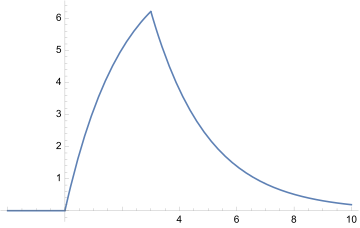
\includegraphics{q7a.png}
				\end{center}
				The plot should also make sense intuitively: for \( t > 3 \), we are taking the convolution across 
				a decaying exponential, so therefore the resulting \( y(t) \) will look that way. For 
				\( t < 0 \) the convolution is zero because there is no overlap. For \( 0 < t < 3 \), the 
				area is growing because as we increase \( t \), more area between the two functions overlap, up to a
				maximum at \( t = 3 \). 
			\end{solution}
		\item Compute the cross correlation of \( x(t)  \) and \( g(t) \), \( R_{x, g}(t) = 
			x(t) \circ g(t)\), then sketch your result.

			\begin{solution}
				The definition of the cross correlation formula is 
				\[
				x(t) \circ g(t) = \int_{-\infty}^{\infty} x(\tau) g( t + \tau) \diff \tau  
				\] 
				We will apply a very similar trick to the previous portion: since \( x(\tau) \) is nonzero 
				on \( [0, 3] \), then we can restrict the domain, and use the fact that \( x(\tau) \) is 
				constant on this interval: 
				\[
				R_{x, g}(t) = 2\int_{0}^{3} g(t + \tau) \diff \tau 
				\] 
				Now, the integral sweeps over the interval  \( [t, t + 3] \). Therefore, for \( t < -3, \) then we 
				have \( R_{x, g}(t) = 0 \). For \( -3 \le  t \le  0 \), then the integral goes from 
				\( [0, t + 3] \), so the result is: 
				\[
				R_{x, g}(t) = 2 \int_{0}^{t + 3} g(\tau) \diff \tau  = 4(1 - e^{-(t + 3) /2})
				\] 
				Then, for \( t > 0 \), we have: 
				\[
				R_{x, g}(t) = 2 \int_{t}^{t + 3} g(\tau) \diff  \tau = 4e^{-(t + 3) /2}(e^{3 /2} - 1)
				\] 
				Therefore, we can write:
				\[
				R_{x, g}(t) = \begin{cases}
					0 & t < -3\\
					4(1 - e^{-(t + 3) /2}) & -3 \le t\le 0\\
					4e^{-(t + 3) /2}(e^{3 /2} - 1) & t>0
				\end{cases}
				\] 
				As for the sketch: 
				\begin{center}
					\includegraphics{q7b.png}
				\end{center}
			\end{solution}
		\item Compute the cross correlation of \( g(t) \) and \( x(t) \), \( R_{g, x}(t) = g(t) \circ x(t) \), then 
			sketch your result. 

			\begin{solution}
				Instead of computing the entire thing again, we make use of the identity that 
				\[
				x(t) \circ g(t) = g(t) * x(-t)
				\] 
				So this means that \( R_{g, x}(t) = R_{x, g}(-t) \). Therefore, making the substitution 
				\( t \to -t \) in the formula for \( R_{x, g}(t) \) above, we get: 
				\[
				R_{g, x}(t) = \begin{cases}
					0 & t > 3\\
					4(1 - e^{-(3 - t) /2}) & 0 \le t \le 3\\
					4e^{-(3 - t) /2}(e^{3 /2} - 1) & t < 0
				\end{cases}
				\] 
				Plotting: 
				\begin{center}
					\includegraphics{q7c.png}
				\end{center}
			\end{solution}
		\item Briefly describe how convolution and cross correlation of two signals are related but very different.  

			\begin{solution}
				Convolution and correlation are the same in the sense that they both calculate some relationship 
				between two functions \( f \) and \( g \) by taking pairwise products across the function. 
				Convolution flips the second function \( g \) and slides it across \( f \), whereas cross correlation 
				doesn't do any flipping and just slides \( g \) across \( f \) and computes the product. 
			\end{solution}
	\end{enumerate}
\end{document}
